%!TEX root = ../main.tex


%(3) In data lake storage,  it is challenging to perform  optimization like in a database because the computing engine is always decoupled with the storage. Hence, it is critical to consider how to incorporate an optimizer in the storage engine, so as to optimize system performance.


% Third,  we build an intelligent data lake optimizer \brain at the storage-side that focuses on optimizing the data layout in the storage, so as to improve the resource utilization as well as  query performance. Many recent works~\cite{}  have focused on using machine learning techniques to  optimize database systems, including the knob tuner, query optimizer etc. For the data lake system with the disaggregated storage, we think that it is a promising direction to design an optimizer and we conduct the following two attempts. We design a reinforcement learning based automatic compaction module  to decide whether to compact small files considering the system state at a certain system status, so as to \cc{improve the block utilization while keeping the system running smoothly.} We also build a predicate-aware partitioning model that is utilized to judiciously distribute data to storage blocks to reduce the number of blocks to be visited, so as to improve the query efficiency. 

\section{Lakebrain optimization} 
\label{sec:lakebrain}




%\cc{Below is very hard to follow! what is talking about?where is the partition? what is the connection with the above?}


%LakeBrain's design is kept simple for ease of extension and support for different applications. It consists of three components: a statistics collector, the core optimization logic, and an executor. The statistics collector gathers system configurations, environment variables, and workload history, while the core optimization logic employs heuristic rules, probabilistic models, and machine learning algorithms to suggest the best strategy candidates. The executor then deploys the chosen strategy, with its effects being collected as feedback by the statistics collector for future optimization.


%To demonstrate the value of a data lake storage optimizer, we have developed two LakeBrain applications: auto compaction and predicate-aware fine-grained partitioning. These use cases will be explained in detail in the following section.

Optimizing  query processing over large-scale data is significant in data warehouse and big data systems, as discussed in~\cite{oracle, tere, survey, eltabakh2021not, pandit2015accelerating, armbrust2015spark}. However, for the \sys system with
complicated storage-disaggregated architecture, it is challenging to optimize the query performance and resource usage. The reasons are two-fold. First, it is hard to capture the entire environment about the compute and storage cluster as well as the queries executed by other engines simultaneously. Second, even though all the environment data is available, it is still hard to optimize because of the large search space due to the large number of tunable and interdependent variables~\cite{jindal2021microlearner}.

\cc{how to solve the two challenges still not clear!}

To address the challenges, we present~\brain, a novel data lake storage optimizer that aims to optimize the  the data layout at the storage-side, so as to improve the resource utilization as well as  query performance.
Unlike query engine optimizers that focus on join order and cardinality estimation~\cite{rtos, deepdb, naru}, \brain aims to optimize data layout in storage, which is key to improve both query performance and storage resource utilization in a storage-disaggregated design. In this Section, we mainly focus on two cases, $i.e.,$ automatic compacting small files  and judiciously partitioning tables to improve the resource utilization improve the query performance.
Next, we will illustrate the above aspects in detail.

\subsection{Automatic Compaction}~\label{subsec:compaction}
In a streaming application scenario, data ingestion and transactions often result in numerous small files, leading to low query performance on merge-on-read (MOR) tables. 
A typical method is to compact files statically using rule-based methods such as setting a time window or a data size threshold~\cite{iceberg,hudi}.
In this part, \brain  designs the automatic compaction to combine these small files into fewer and larger ones, so as to  improve the block utilization  as well as query performance.

The block utilization at a certain state $t$ is defined by $\frac{\sum_{i=1}^{n}f_t^i}{K \times  \sum_{i=1}^{n}\lceil \frac{f_t^i}{K}\rceil}$, where $n_t$ denotes the number of files at the state, $f_t^i$ denotes the size of each file and $K$ is the block size.
 As streaming data is continuously ingested,  we are likely to frequently determine whether to merge small files.
  However, considering a certain state in the system, we cannot simply  compact files when the block utilization is low because both compaction and data ingestion require commits, which may have conflicts, leading to compaction failure or ingestion slow down. On top of that, compaction consumes relatively large amount of computing resource. Moreover,  there exist a number of system parameters \cc{($e.g.,$ file ingestion speed, target file size, etc any more???) } that have impact on  the system.  The action ($i.e.,$ whether to merge files) at each state will change some parameters, but it does not purely influences current system situation, but also future states. 
  Hence, compaction aims to achieve long-term rewards, $i.e.$, co-optimizes the query performance  and storage utilization at the end.
  

Therefore, we propose a reinforcement learning framework that can well capture the relationship between system parameters of each state and the long-term benefit (considering the future system states) of conducting the compaction or not. 
To be specific, as shown in  Figure~\ref{fig:rl}, 

\noindent \underline{\textit{Agent}} can be taken as our automatic compaction module that receives the \texttt{reward} (resource utilization) and \texttt{state} (system parameters) from the \texttt{environment} (the storage system). Then it updates the policy network ($e.g.,$ Deep Q-Network~\cite{dqn,dqn2}) to guide whether to conduct the compaction operation so as to maximize the long-term reward.

\noindent \underline{\textit{State}} denotes the current state of the storage system, described by \cc{many} features, for example, among which \cc{XX} are significant ones closely  related to the compaction problem. These features will be encoded as the input of the policy network.

\noindent \underline{\textit{Reward}}  reflects whether the compaction  has a positive or negative impact on the system and the extent of the impact. Specifically, if the compaction succeeds, the reward is  computed by the improvement of the block utilization. If it fails, the reward is the minus of the number of partitions that participant this compaction.

\noindent \underline{\textit{Action}} denotes whether we conduct the compaction at each state, which is the output of the policy network. If we decide to compact, we will \cc{XXXX}.


Overall, the training process is that given each state in the system, when acting the compaction or files are keeping ingested, the state will change and we can observe the reward provided by the environment. We will store these experiences (previous states, action  and reward triples) and allow the agent to reuse them to train the policy network of the agent.
This process repeats until the model converges. For inference, as the streaming data comes continuously, we can trigger the trained RL model every few moments to determine whether to  compact the files.


%As discussed above, file compaction aims to find the optimal strategy for compacting files that can improve query execution time or increased block utilization\footnote{not mentioned above} in storage. To achieve this goal, the optimization process employs two algorithms\footnote{two algorithms or steps?}: particle swarm optimization (PSO)\footnote{is there a citation? } and reinforcement learning (RL).

%PSO is used to search for the global optimum, a population-based method that doesn't require assumptions about the relationship between tunable parameters and query performance. The goal is to obtain an approximately optimal solution within a limited time.  \cc{Not clear!! We should say what is the entire problem, and why and how to split it into two steps.}


%\cc{Also not clear!! We should introduce what is the problem and the optimization goal that fit the paradigm of RL. Then define the critical components of RL and illustrate that.} RL secondly finds a more sophisticated policy based on the states of the data lake environment. The optimization process involves considering a set of discrete compaction configurations within the action space. Since the state space is continuous, a function approximation method is preferred. The stability of the training process is critical due to the high degree of variability in query performance in a distributed environment, so proximal policy optimization (PPO) is applied.

\begin{figure}[htbp]
	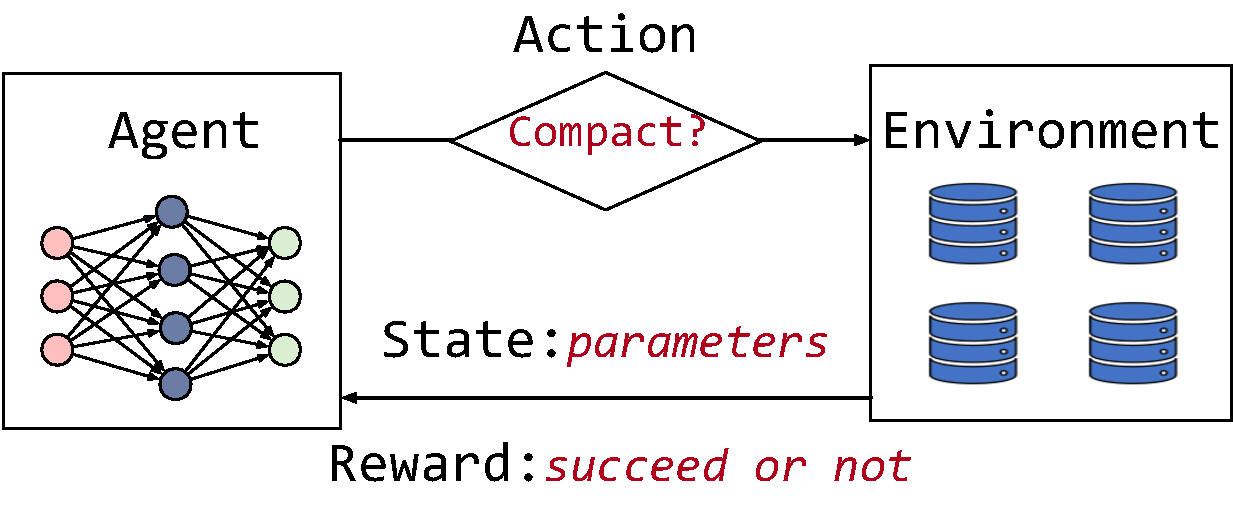
\includegraphics[scale=0.33]{figures/rl}
	\centering
	\vspace{-1.5em}
	\caption{Automatic Compaction using RL.}
	\label{fig:rl}
	\vspace{-1em}
\end{figure}

%A deep neural network (DNN) is used to approximate the policy and the value function, with a shared feature backbone network that covers both global and local characteristics of the states. The output from the feature network is processed by two fully connected networks to compute the policy output and the action value. The actor and critic are alternatively updated after collecting new trajectories using the latest policy during training.

%Once a desired result is obtained, the numerical output of the compaction strategy is translated into actionable operations by the data lake connector for a specific data lake engine, facilitating the optimization process.






\subsection{Predicate-aware Partitioning}~\label{subsec:partition}


With  data  increasing, we  have to partition the data into different storage blocks such that the query efficiency can be much improved. In practice, users always select a single (or multiple) column as the partition key,  apply   a hash function to the values of the key, and then distribute the data to different blocks based on the partition values. This method is sub-optimal $w.r.t.$ the latency because it may lead to imbalanced data distribution. \brain  designs predicate-aware  method to partition the data in a fine-grained way such that given a query, the \cc{number of blocks or tuples?} to be assessed is minimized, and thus the efficiency is improved.


\begin{figure}[htbp]
	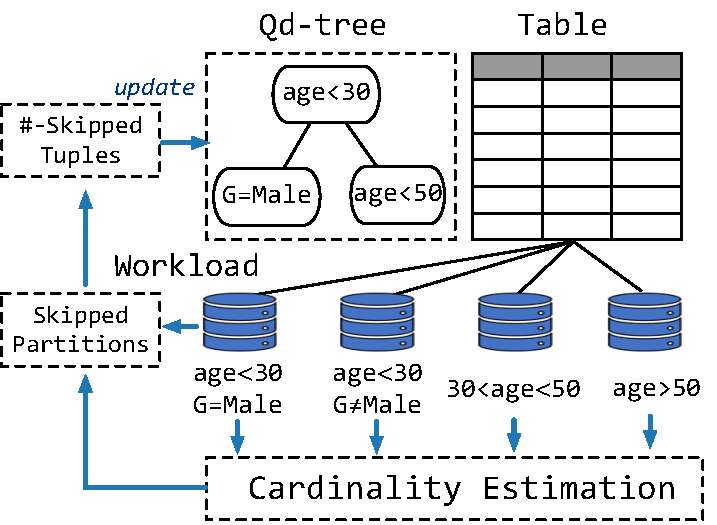
\includegraphics[scale=0.5]{figures/partition}
	\centering
	\vspace{-1em}
	\caption{Predicate-aware Partitioning.}
	\label{fig:partition}
	\vspace{-1em}
\end{figure}


 Specifically, our partition method is based on the query-tree framework~\cite{qdtree}, and additionally leverage the machine learning based cardinality estimation method for optimizing the query tree, so as to find a fine-grained data partition with high query efficiency. 
As shown in Figure~\ref{fig:partition}, given a table $T$ and a query workload $W$ consisting of the pushdown predicates, we will build a query tree, similar to a decision tree where each inner node denotes a predicate in the form of (attribute, operator, literal), where operator includes $\{\leq, \geq, <, >, =, IN\}$. Each leaf node refers to a partition such that when executing $W$, we can skip as many tuples as possible. For example, the leftmost partition contains tuples satisfying $\texttt{age}<30$ \texttt{and} $\texttt{G=Male}$. Given $W$ and the partitions, we can compute how many partitions that we can skip. But in order to compute the number of skipped tuples, we have to know the cardinality of each partition. We can either directly compute the cardinality, or sample for estimation, which is time-consuming or not accurate enough. Hence, we can use AI-driven cardinality estimation methods~\cite{face, e2e, naru, deepdb} to estimate the cardinality accurately and efficiently via learning the data distribution. In practice, we use the sum-product network~\cite{deepdb} as the estimator. 
%Optimizing data partitioning~\footnote{* we should first say what is the data partition problem (does the previous section mention it?)} involves assigning records to storage blocks in the most efficient manner possible, thereby reducing the number of blocks accessed during queries. Our partitioning approach is based on the query-tree framework [43], and utilizes a sum-product network (SPN) probabilistic model [19, 26, 31] to model the distribution of the data in LakeBrain. This is done in order to ensure fast inference speed and avoid repeatedly scanning the datasets.



%The query-tree framework creates a tree-based partitioning strategy using pushdown predicates. Each leaf node represents a partition, and its column ranges are derived from the pushdown predicates used to split its parent nodes.
 %By using probabilistic models to characterize the dataset, we can identify the most suitable partitioning policy. The probabilistic model-based cardinality estimation, as demonstrated in Figure 11, is used to estimate the number of records in each partition, \cc{How?? query-driven or data-driven? both cases should have queries to test} instead of scanning the original data, thereby saving a significant amount of time. This greatly improves the speed of the partitioning optimization algorithm, making it suitable for large-scale systems.

%Additionally, probabilistic models allow us to represent a sequence of datasets with a series of probabilistic models that have a fixed structure but varying parameters. This is achieved by representing a sequence of datasets as a series of multi-dimensional vectors, each representing the learnable variables in the probabilistic model with a fixed length, i.e. a time series. We can then use time series prediction methods to predict future probabilistic models, and use these predictions to estimate the number of records in a partition during partitioning optimization\cc{like a magic}.




%To implement the optimized data layout, we introduce a partitioning mechanism that saves data in fine-grained partitions based on the partitioning strategy. Additionally, we have implemented an evaluator that skips irrelevant partitions by checking the overlap between pushdown predicates and the column ranges in each partition. For numerical columns, the range can be represented as lower and upper bounds, which are well-handled by many data formats. For categorical columns, we either record its range or its complement using "IN" or "NOT IN" predicates. The effectiveness of this predicate-aware partitioning approach is evaluated in section 7.2, where the test results show exceptional performance.
